%28/10 - Fátima Sánchez Cabo
\chapter{Introducción a la genómica: caracterización del genoma mediante NGS}
\section{Introducción a la genómica traslacional}
\subsection{Definición e importancia de la genómica}
La genómica, el estudio integral del ADN y de la estructura, función y dinámica de los genomas, representa un pilar fundamental en la biología moderna. Marcó un cambio de paradigma, pasando de un enfoque reduccionista en biología - donde se estudiaban componentes individuales y de manera aislada - a una perspectiva integradora que analiza las interacciones y relaciones entre los distintos elementos biológicos. Esta transición permitió evolucionar de la genética clásica, basada en hipótesis concretas, hacia la genómica, que integra análisis de datos masivos sin necesidad de preguntas iniciales específicas, aunque sí en constante búsqueda de respuestas biológicas complejas.

En el marco del dogma central de la biología, las “ómicas” representan tres niveles de estudio: la genómica (centrada en el ADN), la transcriptómica (ARN) y la proteómica (proteínas). Este curso se enfoca en la genómica, ya que la información genética determina las funciones bioquímicas y, por ende, los fenotipos de los organismos. Gracias a avances recientes, ahora es posible inferir la función bioquímica de las proteínas directamente a partir de la secuencia de ADN, sin necesidad de técnicas complejas como la cristalización. Además, herramientas de inteligencia artificial pueden predecir la estructura de las proteínas con precisión, acelerando la interpretación de funciones biológicas.

Las proteínas, incluyendo enzimas esenciales, son los elementos funcionales clave en la biología. La secuencia de aminoácidos en una cadena polipeptídica define sus propiedades funcionales, y, por tanto, conocer la secuencia genética subyacente (el ADN) facilita predecir la función de una proteína. Aunque determinar experimentalmente las propiedades de una proteína es complejo, la secuenciación genómica ha simplificado enormemente este proceso.

La mejora en tecnologías de secuenciación impulsó el \textbf{Proyecto Genoma Humano}, que logró identificar entre 20,000 y 25,000 genes y determinar la secuencia de los aproximadamente 3 mil millones de pares de bases del genoma humano. Este proyecto también fomentó la creación de bases de datos y herramientas para el análisis de datos genómicos, además de abrir el debate sobre los aspectos éticos, legales y sociales (conocidos como ELSI, por sus siglas en inglés), que siguen siendo temas vigentes y complejos en la actualidad.

\paragraph{Evolución de la bioinformática en la genómica}
La bioinformática ha crecido a la par de la genómica en múltiples niveles. Inicialmente, era una \textbf{disciplina} incipiente y se desarrollaba como apoyo experimental; sin embargo, ha evolucionado hasta convertirse en un campo esencial que impulsa la investigación. En cuanto a su \textbf{material, los datos,} la bioinformática ha tenido que adaptarse al fenómeno del big data, pasando de manejar cantidades limitadas de datos a enfrentar volúmenes masivos, propios de la genómica actual. Paralelamente, el \textbf{rol de los bioinformáticos} se transformó, pasando de ser técnicos a científicos de datos y académicos altamente reconocidos en la industria y en la investigación.

\begin{figure}[htbp]
\centering
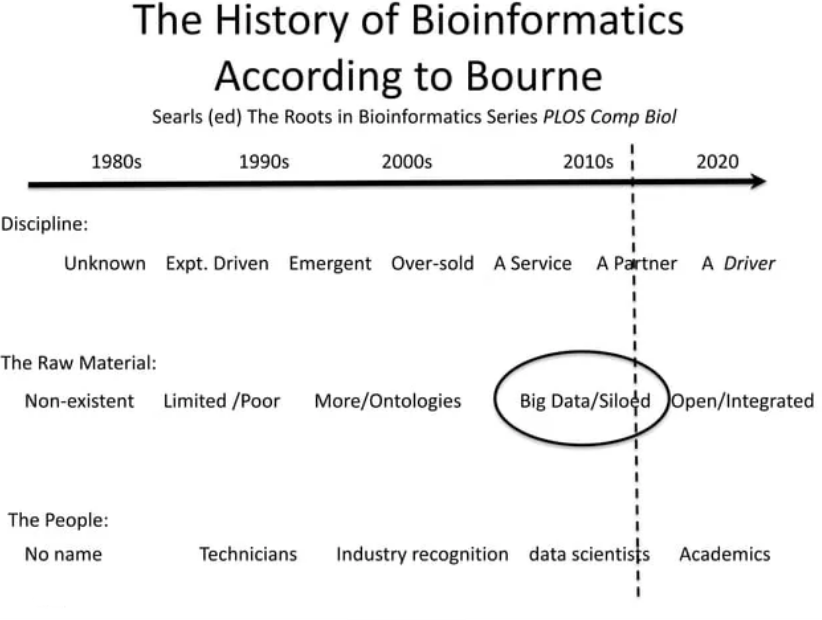
\includegraphics[width = 0.5\textwidth]{figs/history-bioinfo.png}
\caption{Breve historia de la bioinformática en tres niveles: como disciolina, como material que utiliza y como las personas que trabajan en ella. Evolución desde 1980 hasta 2020.}
\end{figure}

\subsection{Avances tecnológicos en secuenciación}
Existen distintos tipos de tecnologías de secuenciación, comúnmente clasificadas en tres generaciones: la primera generación (first generation), la segunda o Next Generation Sequencing (NGS) y la tercera generación. Las dos primeras generaciones se enfocan en la secuenciación de fragmentos cortos de ADN, mientras que la tercera generación permite la lectura de fragmentos largos, facilitando el ensamblaje completo de genomas. Actualmente, uno de los mayores desafíos tecnológicos es detectar variantes de baja frecuencia y realizar secuenciaciones de ADN en células individuales (single-cell sequencing), lo cual tradicionalmente se hacía de forma masiva (“bulk”).

\begin{figure}[htbp]
\centering
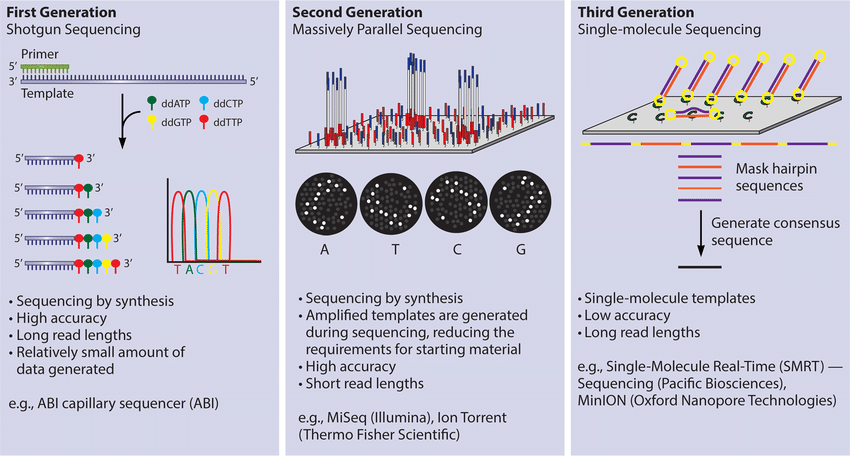
\includegraphics[width = 0.7\textwidth]{figs/sequencing-generations.png}
\caption{Las tres generaciones de secuenciación y su forma de actuar.}
\end{figure}

A medida que el costo de la secuenciación ha disminuido y la capacidad de almacenamiento ha mejorado desde 1990, los datos generados también han crecido exponencialmente. En un experimento de secuenciación, los costos abarcan tanto la secuenciación en sí como el procesamiento bioinformático, el reporte y el almacenamiento de los datos. La comunidad científica y muchos journals requieren que los datos de proyectos financiados públicamente estén disponibles en bases de datos accesibles, lo que asegura la transparencia y el acceso a esta información valiosa. Para obtener una cobertura de calidad, el ADN suele secuenciarse al menos 30 veces, lo que genera archivos de gran tamaño, como los archivos FastQ, que almacenan información de secuencia y calidad para cada base.

\subsection{Procesos de llamada y priorización de variantes}
Los datos de secuenciación se procesan en pipelines bioinformáticas que comienzan con archivos FastQ normalmente comprimidos y pasan por varias etapas: control de calidad, alineamiento y llamada de variantes (variant calling). Las variantes identificadas pueden incluir cambios de nucleótidos, variaciones en el número de copias de segmentos genómicos (copy number variation) o reordenamientos estructurales.

\begin{figure}[htbp]
\centering
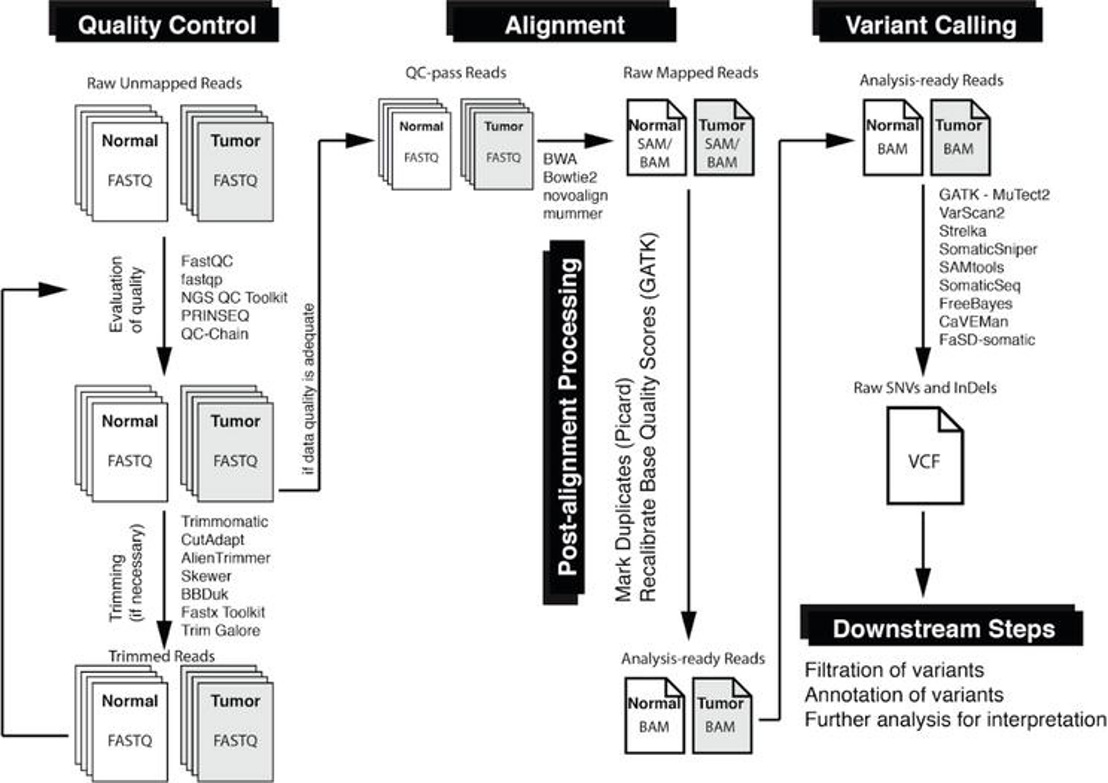
\includegraphics[width = 0.7\textwidth]{figs/bioinfo-pipeline.png}
\caption{Esquema de la pipeline que se sigue en bioinformática para la llamada de variantes.}
\end{figure}

La priorización de variantes se basa en factores como el impacto funcional, la frecuencia alélica en la población y la asociación con enfermedades. Sin embargo, muchas variantes requieren validación experimental, frecuentemente en modelos animales como ratones, para corroborar su relevancia funcional. El proceso de filtrado inicial se enfoca en variantes en exones de genes candidatos, analizando su frecuencia, patogenicidad y modelo de herencia; en caso de no hallarse variantes relevantes, se amplía el análisis a variantes oligogénicas o no codificantes.

\begin{figure}[htbp]
\centering
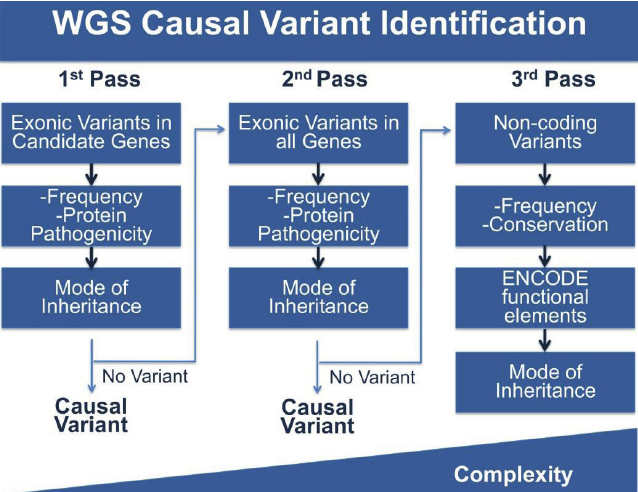
\includegraphics[width = 0.5\textwidth]{figs/variant-priorization.png}
\caption{Ejemplo de la priorización de variantes.}
\end{figure}

\subsection{Genómica en medicina de precisión}
La genómica ha transformado el enfoque de la medicina de precisión, permitiendo identificar enfermedades con bases genéticas, ambientales o una combinación de ambas. Algunas variantes genéticas confieren una predisposición a enfermedades sin ser causantes directas, lo cual es crucial para inferir relaciones causales y acelerar ensayos clínicos mediante la integración de grandes volúmenes de datos. Estas variantes pueden clasificarse en germinales (heredadas) o somáticas (adquiridas).

\begin{figure}[htbp]
\centering
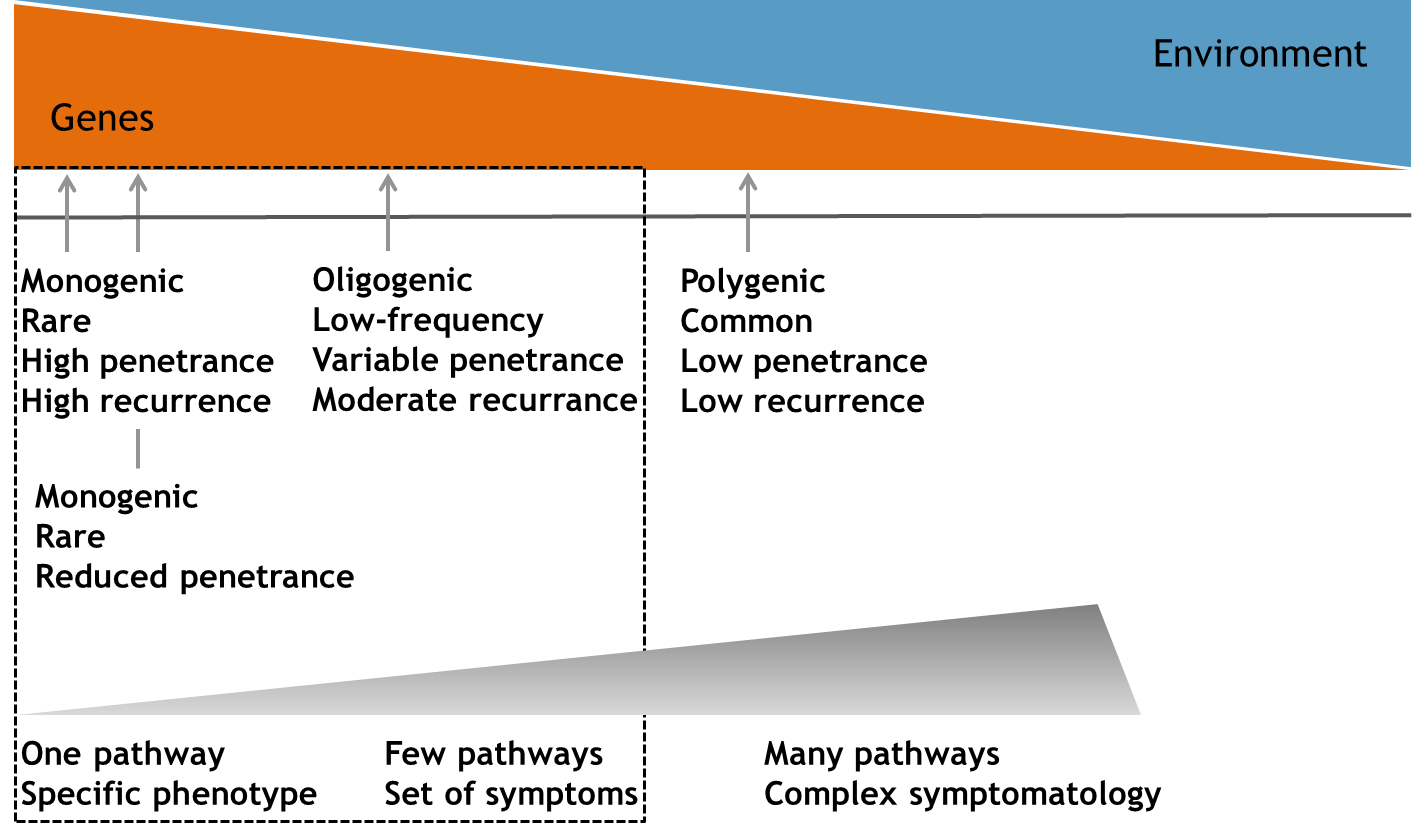
\includegraphics[width = 0.5\textwidth]{figs/genetic-environment.png}
\caption{Representación gráfica de la relación entre enfermedades con base genética, ambientales o una mezcla de ambas.}
\end{figure}

En medicina de precisión, la genómica es solo una capa de datos entre muchas. Para una comprensión holística de la salud y la enfermedad, es necesario combinarla con información de otras “ómicas” como la transcriptómica, epigenómica, proteómica, metabolómica, y datos de microbioma. Además, los datos clínicos y epidemiológicos también forman parte del ecosistema de \textbf{Big Data Biomédico}, que actualmente se maneja mediante técnicas avanzadas de computación en clusters HPC, computación en la nube y algoritmos de GPU.

\begin{figure}[htbp]
\centering
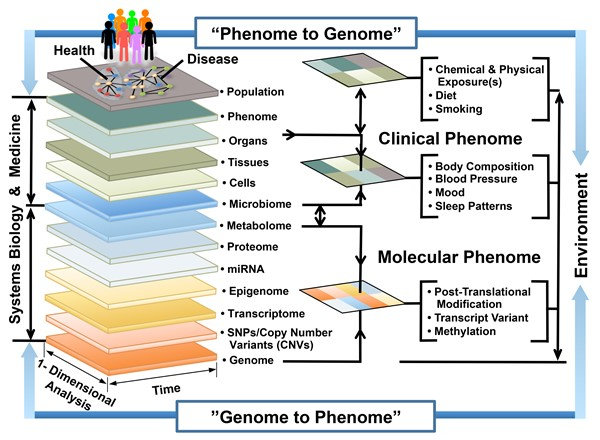
\includegraphics[width = 0.7\textwidth]{figs/bigger-picture-bioinfo.jpg}
\caption{Esquema representando el dibujo general de la bioinformática.}
\end{figure}

Varias bases de datos públicas permiten estudiar la transición entre salud y enfermedad. El estudio de Farmingham, por ejemplo, lleva más de 70 años recolectando datos de factores de riesgo cardiovascular en más de 15,000 participantes. En Reino Unido, el Biobank y, en Estados Unidos, la iniciativa All of Us, también representan recursos de gran envergadura. En España, el CNIC (Centro Nacional de Investigaciones Cardiovasculares) realiza el estudio PESA (Progression of Early Subclinical Atherosclerosis), que ha contribuido a identificar factores predictivos de aterosclerosis subclínica mediante el estudio multiómico, generando nuevos indicadores con un mayor poder predictivo de la formación de placas de colesterol.

\paragraph{Epigenética y la medición de la edad biológica}
El perfil de metilación del ADN es un factor epigenético que puede modificar la expresión genética y se ha utilizado para calcular la “edad biológica” o epigenética de una persona, lo que puede servir como predictor de esperanza de vida y salud. Al comparar estos perfiles con la edad cronológica, sexo y otros factores, se obtiene información sobre el envejecimiento y el riesgo de enfermedades, facilitando el desarrollo de estrategias de salud personalizadas.

\subsection{Resumen}
La genómica ha liderado una revolución científica en el siglo XX, evolucionando desde el estudio de componentes individuales hasta una perspectiva integral de sistemas biológicos y de investigación basada en datos masivos. La bioinformática se ha convertido en una disciplina central en el análisis genómico y predicción de estructuras proteicas, impulsada por el Proyecto Genoma Humano y el desarrollo de tecnologías de secuenciación. Los avances actuales buscan no solo la secuenciación del ADN, sino también la integración de estos datos con datos epidemiológicos y moleculares para obtener una comprensión más profunda de la salud y la enfermedad. Así, el Proyecto Genoma Humano fue decisivo para sentar las bases de tecnologías de secuenciación, el desarrollo de la bioinformática en sí y el uso social e industrial de los datos ómicos.

La identificación de características genómicas relevantes causales de rasgos/enfermedades se basa en la anotación de variantes en bases de datos y en estudios poblacionales: hay margen de mejora y un gran éxito de la ciencia colaborativa. Hoy en día, los principales proyectos tratan no sólo de secuenciar el ADN, sino de integrar esta información con datos epidemiológicos y otros datos moleculares para comprender mejor la salud y la enfermedad.
Las enfermedades, en función de su base genética, pueden clasificarse en monogénicas (mendelianas), oligogénicas (ej., cardiopatías familiares) y complejas (evaluadas mediante puntuaciones de riesgo poligénicas). Esta clasificación permite avanzar en la medicina de precisión, abordando enfermedades desde su origen genético para ofrecer intervenciones de salud más efectivas y personalizadas.
